%% grundlagen.tex
%% $Id: grundlagen.tex 28 2007-01-18 16:31:32Z bless $
%%

\chapter{Grundlagen}
\label{ch:Grundlagen}
%% ==============================

In diesem Kapitel werden grundlegende Terminologien, die für das Verständnis der Arbeit relevant sind erläutert.
Dazu werden zunächst psychologische Hintergründe der Geselligkeit betrachtet und
dann Smartphones und Aspekte des Android Betriebssystems erklärt, die für die Betrachtung von Social Media und Instant Messaging relevant sind.
Am Ende des Kapitels werden verwandte Arbeiten aufgezeigt.

%% ==============================
\section{Persönlichkeitspsychologie}
%% ==============================
\label{ch:Grundlagen:sec:Abschnitt1}

Zentral für diese Arbeit ist die Geselligkeit eines Menschen.
Wissenschaftlich fällt das Betrachten dieser Persönlichkeitseigenschaft in den Bereich der Persönlichkeitspsychologie,
oft auch Differenzielle Psychologie genannt. 
Dieser Zweig der Pychologie beschäftigt sich mit den Unterschieden zwischen verschiedenen Personen, 
basierend auf Funktionen, Fähigkeiten und Verhalten, deren Ursprünge und der Konsequenzen der selben.
Sie bildet eine Grundlage für praktische Anwendung unter anderem im klinischen oder pädagogischen Kontext.
\par

Historisch begonnen hat das Fachgebiet mit der Intelligenzforschung und Quantifizierung, 
die auch Heute noch ein wichtiger Grundpfeiler der Differenziellen Psychologie ist.
Im Laufe der Zeit kamen weitere Thematiken hinzu wie Temperatmenteigenschaften, Einstellungen und, für diese Arbeit relevant, Sozialverhalten.
\par

Bisher konnte sich keine allgemeine, allumfassende Persönlichkeitstheorie durchsetzten, sondern es gibt eine breite Masse an verschiedenen Ansätzen und Menschenbildern, die von verschiedenen Theoretikern unterstützt werden
\ignore{ Beispiel Sigmund Freund?}
Im Rahmen dieser Arbeit wird mit dem "`Big Five"' Persönlichkeitsmodell gearbeitet, das im deutschsprachigen Raum auch manchmal das "`Fünf Faktoren Modell"' genannt wird.
Es ist, neben dem Myers-Briggs Type Indicator, eines der bekanntesten, meistgenutzten Modelle und wird der Forschung weithin anerkannt.
Das Big Five Modell bietet sich speziell für diese Arbeit an, da es bei diesem Modell sehr einfach ist, nur den Geselligkeits Aspekt und direkt zusammenhängende Aspekte zu betrachten.

\subsection{Big Five Modell}

Nach dem Big Five Modell existieren fünf Hauptdimensionen, die die Grundlage für die Persönlichkeit eines Menschen bilden.
Jeder Mensch lässt sich demnach auf 5 Skalen einordnen, wie sehr die folgendende Eigenschaften bei ihr ausgeprägt sind.

\begin{itemize}
  \item Openness to Experience (Offenheit für Erfahrungen)
  \item Neuroticism (Neurotizismus)
  \item Conscientiousness (Gewissenhaftigkeit)
  \item Agreeableness (Verträglichkeit)
  \item Extraversion
\end{itemize}

Das Big Five Modell verfolgt hierbei einen lexikalischen Ansatz: 
Persönlichkeitsmerkmale schlagen sich in der Sprache der sprechenden Person nieder.
Eine Faktorenanalyse über eine Liste von 18.000 Begriffen ergab die fünf oben stehenden Faktoren.
Diese bleiben über die Lebensspanne stabil und können in den verschiedensten Kulturen beobachtet werden.

\subsection{NEO-PI-R}

Der "`NEO - Personality Inventory - Revised"' ist ein Persönlichkeitstest, der das Big Five Modell implementiert.
Der NEO-PI-R ist eine 1990 erstmals veröffentlichte überarbeitete Version des NEO-Pi's von 1978 und hat seitdem mehrere Aktualisierungen bekommen. Die aktuellste Version ist von 2010.
Basierend auf 241 Aussagen, zu denen die Probandin mit 5 Abstufungen von "`Starke Ablehnung"' bis "`Starke Zustimmung"' ihre Meinung darlegt, legt der Test die 5 Hauptfaktoren plus jeweils 6 Unterfacetten dar.
Die 6 Facetten des für diese Arbeit relevanten Extraversion Faktors sind:

\begin{itemize}
  \item Warmth (Herzlichkeit)
  \item Gregariousness (Geselligkeit)
  \item Assertiveness (Durchsetzungsfähigkeit)
  \item Activity (Aktivität)
  \item Excitement-Seeking (Erlebnishunger)
  \item Positive Emotions (Frohsinn)
\end{itemize}

Im Rahmen dieser Arbeit soll der Fokus vorallem auf der Geselligkeitsfacette liegen.

%% ==============================
\section{Smartphones}

\label{ch:Grundlagen:sec:Abschnitt2}


Als Smartphone wird allgemeinhin ein Mobiltelefon bezeichnet, das zusätzlich zu den herkömmlichten Funktionalitäten eines Mobiltelefons wie Anrufe und SMS-Versand über verschiedene Features eines Personal Computers verfügt. 
Ausschlaggebend für die Klassifikation ist unteranderem das Vorhandensein eines mobilen Betriebssystems.
Typische Smartphonefeatures sind Internetfähigkeit, Touchscreen und die Möglichkeit ohne große Umstände Zusatzprogramme von Drittherstellern zu installieren.
Diese Zusatzprogramme werden im Weiteren als Applikationen, oder kurz Apps, bezeichnet.
\par

Smartphones und mit ihnen das Mobile Web sind inzwischen ein wichtiger Faktor geworden:
2015 besaßen 80\% der Internetnutzer zwischen 16 und 64 ein Smartphone. 
Damit ist das Smartphone das zweitrelevanteste Zugangsgerät hinter den konventionellen Computern, also Laptops und Desktop Rechnern, die mit zusammen 91\% an der Spitze steht\cite{globalwebindex}.
\par

Es gibt eine Vielzahl an verschiedenen Betriebsystemen mit einen Smartphone ausgestattet sein kann.
Jedoch ist der aktuelle Stand, wie in Abbildung \ref{fig:marktanteil} zu sehen, dass der Markt von nur zwei Firmen dominiert wird.
Googles Android Betriebssystem, das mit 80.7\% Marktanteil von neu abgesetzten Geräten dominant an der Spitze steht
und Apples iOS, das mit 17.7\% noch knapp mehr als ein sechstel der Smartphoneverkäufe aufzuweisen hat.
Dahinter liegen auf den Plätzen drei und vier Microsofts Windows und Blackberry mit 1.1\% und 0.2\%\cite{smartphonemarktanteil}.
Dementsprechend wird sich diese Arbeit auf das Android Betriebssystem fokussieren.

\ignore{todo: insert pdf graphic}
\begin{figure}[h]
    \centering
    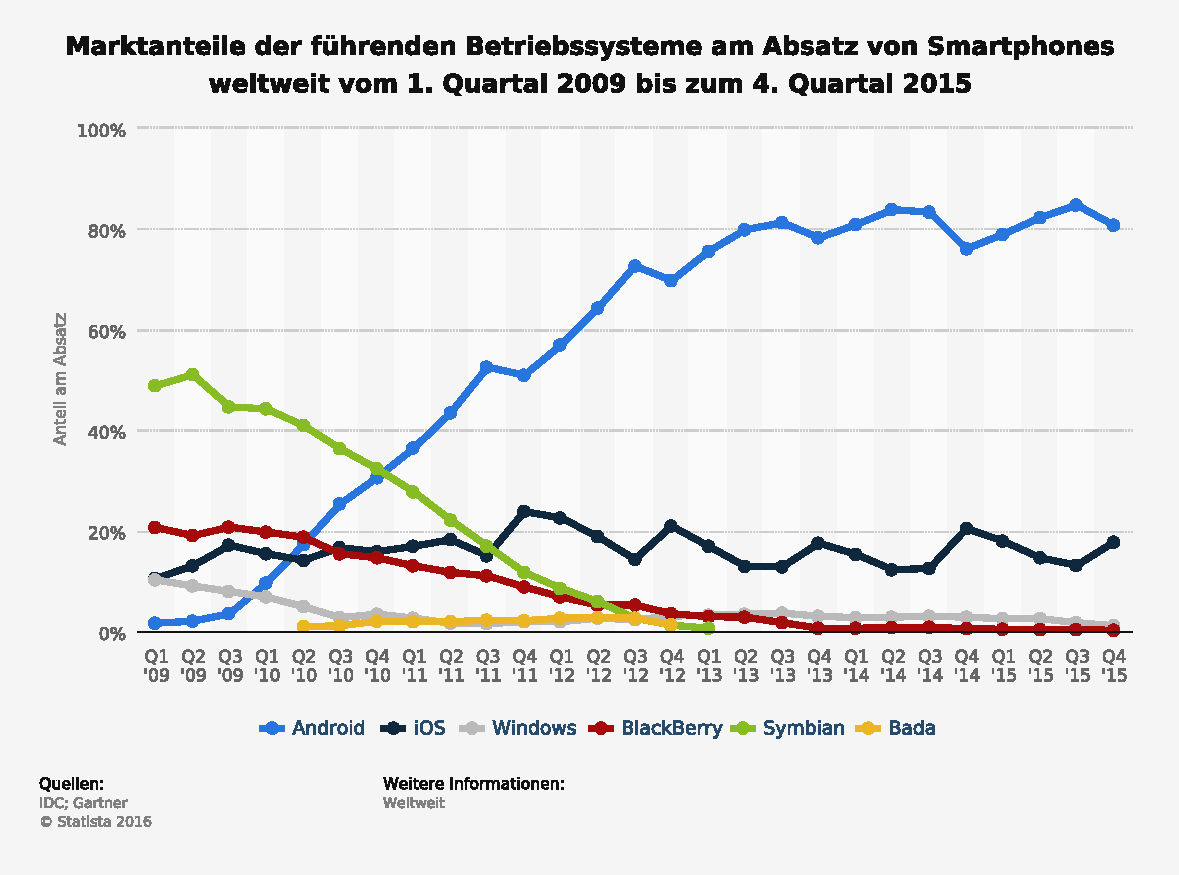
\includegraphics[width=\textwidth]{images/statistic_id73662_marktanteile-der-smartphone-betriebssysteme-am-absatz-weltweit-bis-q4-2015.pdf}
    \caption{Marktanteile der Smartphone Betriebssysteme am Absatz weltweit}
    \label{fig:marktanteil}
\end{figure}


\subsection {Android NotificationManager}

Notifications sind die vom Android Betriebssystem vorgesehene Art und Weise, 
wie eine Applikation die Nutzerin über einen Vorfall aufmerksam macht, während die Applikation nicht im Vordergrund ist.
Dies kann zum Beispiel im Falle der Signal Messenger App eine eingetroffene SMS sein,
oder der erfolgreiche Abschluss eines Updates vom Google Play Store.
Eine gepostete Notification taucht im Allgemeinen zunächst als kleines Pop-up am oberen Bildschirmrand auf und wird dann in die 
Notification Area (siehe Abbildung \ref{fig:notificationarea}) abgelegt.
Durch das Öffnen des Notification Drawers (siehe Abbildung \ref{fig:notificationdrawer}) kann eine detailiertere Ansicht aller ungelesenen Notifications geöffnet werden und gelesene beziehungsweise nicht relevante Notifications entfernt werden 
\cite{androidnotification}.


\begin{figure}%[!htb]
\begin{minipage}{\textwidth}
\centering
  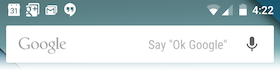
\includegraphics[width=0.75\textwidth]{images/notification_area.png}
  \subcaption{Notification Area\cite{androidnotification}}
  \label{fig:notificationarea}
\end{minipage}
\vfill
\begin{minipage}{\textwidth}
\centering
  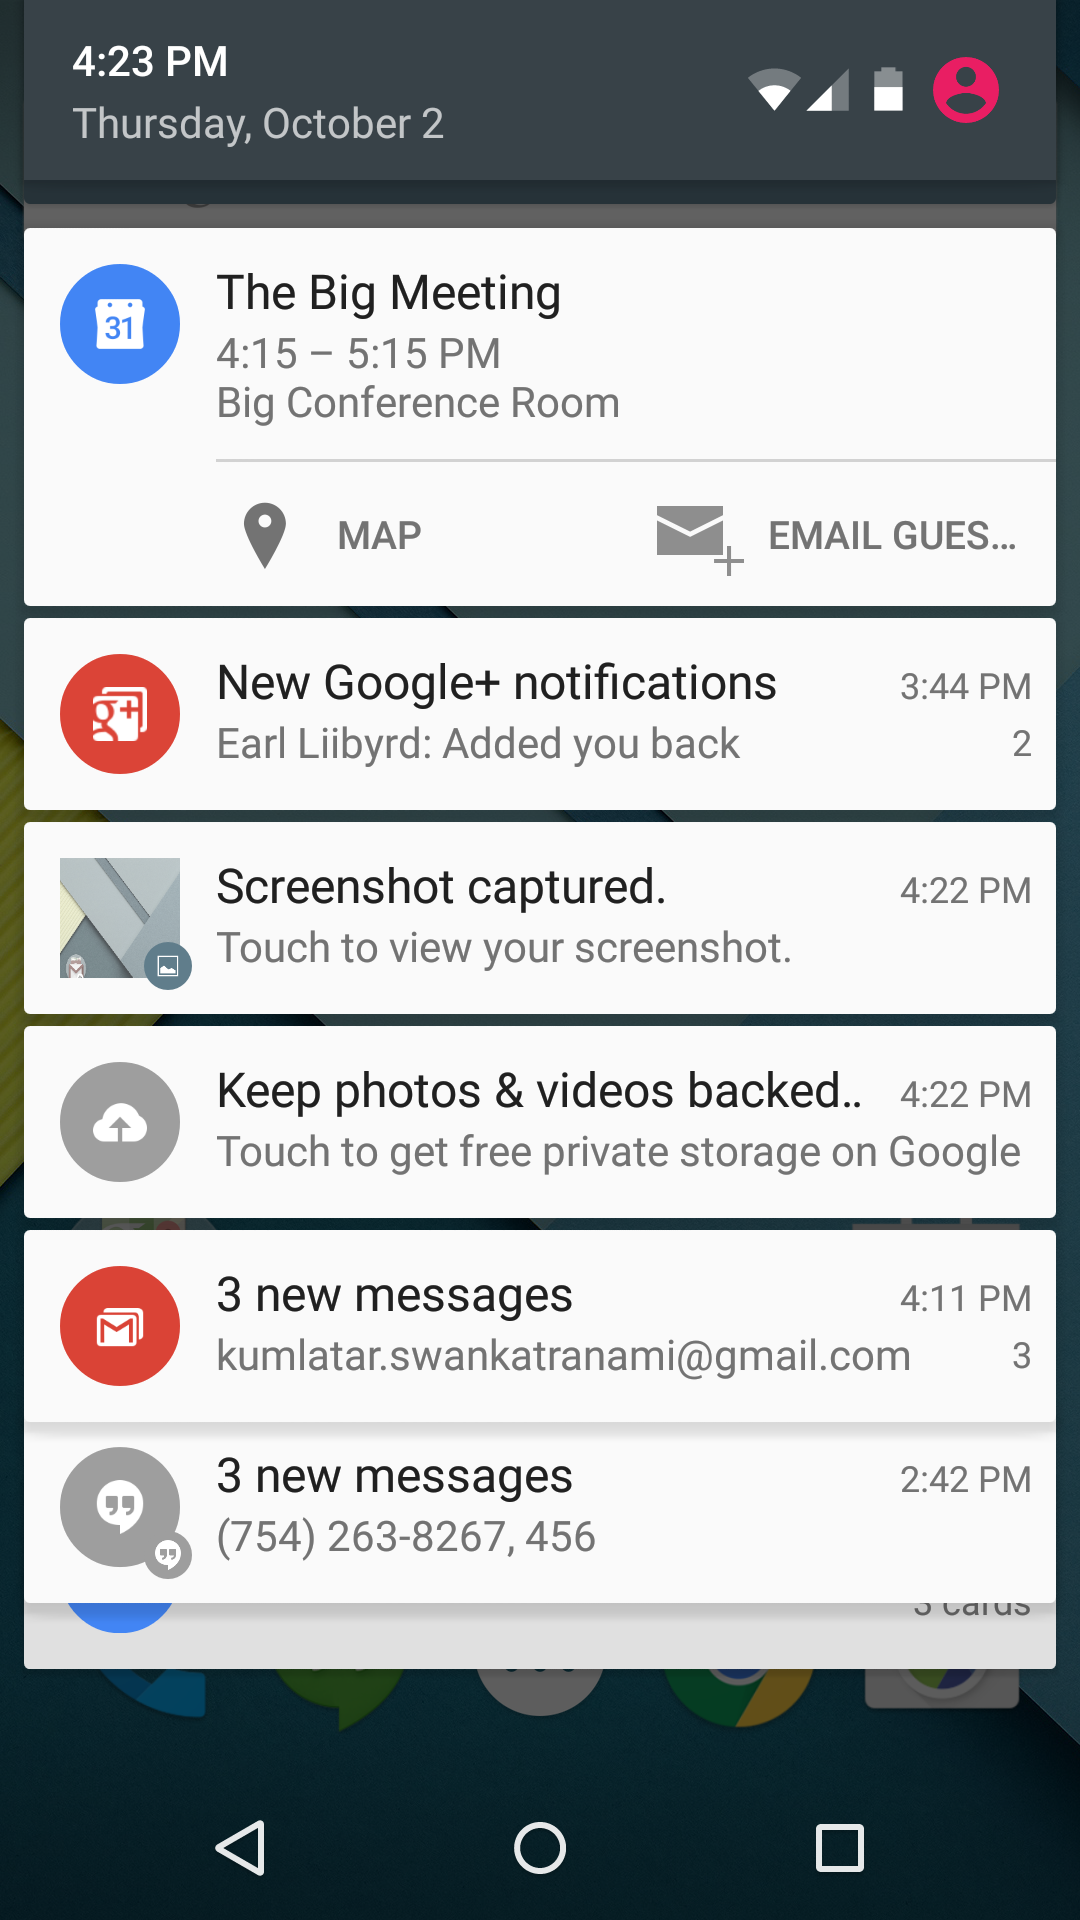
\includegraphics[width=0.75\textwidth]{images/notification_drawer.png}
  \subcaption{Notification Drawer\cite{androidnotification}}
  \label{fig:notificationdrawer}
\end{minipage}
\vspace{-2mm}
\caption{Notificationanzeige in Android}
\label{fig:notAndroid}
\end{figure}

Die Nutzerin kann einstellen, welche Apps Notifications senden dürfen und welche nicht.
So wird ein Spiel, dass konstant auf sich selbst aufmerksam zu machen versucht, wahrscheinlich geblockt,
während dem E-mail Client, der die Nutzerin auf neu angekommene E-mails aufmerksam macht, diese Berechtigung erteilt.
Dementsprechend ist anzunehmen, dass die tatsächlich erhaltenen Notifications die Interessen der Nutzerin widerspiegeln.
\par

Der NotificationManager ist die Stelle im Android Betriebssystem mit denen Apps Zugriff auf alle Notifications bekommen und mit ihnen interagieren können.
Das beinhaltet beliebige Notifications zu erstellen oder gepostete Notifications zu löschen.
An den NotificationManager gebunden werden kann ein sogenannter NotificationListener, mit die Applikation alle an den NotificationManager geschickten Notifications lesen kann.
Dies beinhaltet unter anderem
\begin{description}
    \item {Package} Applikation, die die Notification gepostet hat
    \item {Notification Titel} Titel, oft der Absender der Nachricht
    \item {Ticker} Zusammenfassung der Notification für accessibility services
    \item {Text} Inhalt der Notification
\end{description}
Dies ist eine potenziell leicht zu missbrauchende und falls missbraucht potenziell katastrophale Berechtigung, weshalb die Berechtigung nicht bei der Installation gegeben werden kann, sondern von Hand von der Nutzerin bestätigt werden muss. 


\subsection {Android UsageStatManager}

Der UsageStatManager ist eine Schnittstelle, die Zugang zu vom Betriebssystem gesammelten Daten
und Statistiken bezüglich der Nutzungshistorie des Geräts gibt \cite{androidusagestat}.
Die Methode \textbf{queryUsageStats(int intervalType, long beginTime, long endTime)} gibt eine Liste an UsageStats der verschiedenen Applikationen zurück.
Für jedes Element der Liste erhält man mit der Methode \textbf{getTotalTimeInForeground ()} die Zeit in Millisekunden,
die die App mit dem Package Namen aus \textbf{getPackageName ()} im Vordergrund war.
\par
Die UsageStatManager API benötigt die \textbf{android.permission.PACKAGE\_USAGE\_STATS} Permission.
Diese ist ebenfalls eine priviligierte Berechtigung, die Applikationen zwar beantragen können, die aber nicht bei der Installation erteilt werden kann, sondern nur von der Nutzerin von Hand beantragt werden kann.


%% ==============================
\section{Verwandte Arbeiten}
%% ==============================
\label{ch:Grundlagen:sec:RelatedWork}

Auf dem Gebiet der Persönlichkeitsforschung wurden bereits einige Paper und Studien publiziert,
die das Feld thematisch mit Smartphonenutzungsdaten verknüpfen. 
Verschiedene Arbeiten verfolgen verschiedene Ansätze mit verschiedenen Persönlichkeitsmodellen und betrachten verschiedene Smartphone Features.
In diesem Kapitel sollen einige dieser Arbeiten betrachtet werden und Vor- und Nachteile der verwendeten Methodik betrachtet werden.

\section*{Personality and Self-Esteem as Predictors of Young People’s Technology Use}

In A. Ehrenbergs 2008 im "`CyberPsychology \& Behavior"' Journal erschienenen Artikel "'Personality and Self-Esteem as Predictors of Young People’s Technology Use"' \cite{ehrenberg2008personality}
wird das Ergebnis einer an 200 Universitätsstudentinnen, davon 146 weiblich und 54  männlich, durchgeführte Studie vorgestellt.
Die Probandinnen füllten sowohl einen 60 Fragen umfassenden NEO-FFI Fragebogen aus als auch einen 25 Fragen umfassenden Fragebogen zur Bewertung des Selbstwertgefühls.
Dazu hinzu kam eine Liste an TODO: Selfreported Zeiten werten, dafür wie viele Minuten sie jeweils pro tag mit a\) Telefonaten, b\) SMS und c\) Instant Messaging verbringen.
Abschließend sollten die Probandinnen Aussagen auf ihre Zustimmung hin bewerten, um einzuschätzen wie viel Suchtpotenzial von Technologien für sie ausgeht.
Die Studie fand einen starken Zusammenhang zwischen der Menge an Zeit die mit diesen Technologien verbracht wird und dem persönlichen Suchtpotenzial, Persönlichkeit und Selbstbewusstsein wurden als relativ schwache Indikatoren für die aufgewendeten Zeiten indentifiziert.
\par
Die Wahl von Studentinnen als Zielgruppe macht aufgrund ihrer Rolle als Innovators und Early Adopters von neuen Technologien bei einer solchen Studie sehr viel Sinn.
Auch der Einsatz des Big Five Persönlichkeits Modells als etablierter Standard, implementiert durch den NEO-FFI Fragebogen, ergänzt mit dem Wert für das Selbstwertgefühl sind gut gewählt um eine Ground Truth zu bestimmen.
Im Gegensatz dazu steht die Wahl der Methodik zum Sammeln der Informationen bezüglich der Technologienutzung.
Selfreports sind notorisch unpräzise und voreingenommen.
Auch die Wahl von "`Minuten mit X verbracht"' als (einziger) Messwert für Telefonanrufe, SMS und Instant Messaging ist fragwürdig und, bis auf für Telefonate, kein guter Indikator für die Intensität der Nutzung dieser Kommunikationswege.


\section*{Personality and self reported mobile phone use}

Sarah Butts Artikel "`Personality and self reported mobile phone use"', der im Jahr 2008 im "`Computers in Human Behavior"' Journal veröffentlicht wurde,
behandelt eine Studie, die versucht basierend auf den fünf Persönlichkeitsfacetten des Big Five Modells die Menge und Art der Mobiltelefonnutzung vorauszusagen.
Dazu berichteten 112 Versuchsprobandinnen, davon 78 weiblich und 54 männlich, zwischen 18 und 59 Jahren ihr persönliches Verhalten bezüglich Mobiltelefonen.
Außerdem füllten diese Versuchsprobandinnen den NEO-FFI Persönlichkeitsfragebogen und das Copperfield Self-Esteem Inventory aus.
Der Bericht der Mobiltelefonnutzung beinhaltete folgende Fragen: Zeit aufgewendet für Anrufe, für SMS, für Spiele auf dem Mobiltelefon und für das Ändern von Klingelton beziehungsweise Wallpaper.
Außerdem eine Schätzung wie viele Anrufe getätigt und empfangen wurden, wie viele der ausgehenden Anrufe persönlicher und wie viele geschäftlicher Natur waren und wie viele der eingehenden Anrufe als erwünscht oder unerwünscht eingeschätzt werden.
Zusätzlich wurde erfragt ob SMS oder Anrufe präferiert werden, wie viel Interesse an neuen featuren von Mobiltelefonen besteht und wie lange die Probandin bereits ein Mobiltelefon besitzt.
Die Studie ergab, dass extrovertierte Individuen tendenziell mehr Zeit mit Anrufen und dem Ändern von Klingelton und Wallpaper verbringen.
\par
Wie schon bei der vorangehenden Studie benutzt auch diese Studie den NEO-FFI Fragebogen und ergänzt diesen mit einem Wert für das Selbstwertgefühl der Probandin, was für die Validität dieses Verfahrens spricht.
Die erhobenen Daten sind bedeutend besser gewählt als in der vorangehenden Studie, da sie nicht nur die verbrachte Zeit sondern auch die Anzahl, den Willen der Probandin und deren Präferenz bezüglich SMS oder Anruf erfragt.
Jedoch verlässt sich diese Studie ebenfalls auf Selfreports, was bei Fragen wie zum Beispiel nach der Präferenz zwischen Anruf und SMS sicher sinnvoll ist, aber bei Werten wie Anrufdauer oder Anzahl der Anrufe notorisch unpräzise ist.
Ebenfalls bemerkenswert ist, dass eine Studie, die im Jahr 2008 durchgeführt wurde, also zwei Jahre nach dem Release des ersten Apple iPhones und während des bereits beginnenden Siegeszug der Smartphones, die Features, die Smartphones ausmachen, gänzlich ignoriert.

\section*{The Impact of Personality Traits on Smartphone Ownership and Use}

Die von W. Lane et al 2011 veröffentliche Studie "`The Impact of Personality Traits on Smartphone Ownership and Use"' untersucht den Effekt der Ausprägung der verschiedenen Big Five Persönlichkeitsfacetten.
Von 312 Teilnehmern, davon 60\% weiblich und 40\% männlich, im Alter zwischen 17 und 88 Jahren wurden Werte für die verschiedenen Persönlichkeitsfacetten des Big Five Modells ermittelt und sie sollten sechs Funktionen von Smartphones auf einer Skala von 1 bis 5 bezüglich ihrer Wichtigkeit bewerten.
Diese sechs Funktionen waren Anrufe, SMS, Internet, E-Mail, Musik und Spiele.
Zur Bestimmung der Facettenwerte wurde John's (1991) Big Five Personality Inventory aufgrund seiner geringen Komplexität und schnellen Durchführbarkeit gewählt.
Die Studie ergab, dass Probanden die höher auf der Extraversionsskala lagen, eher Smartphones besaßen und benutzen und relativ viel wert auf die SMS Funktion des Smartphones legen. 
\\
TODO: REVIEW!

\section*{Who’s Who with Big-Five: Analyzing and Classifying Personality Traits with Smartphones}

G. Chittaranjan et al stellen in ihrem Paper "`Who’s Who with Big-Five: Analyzing and Classifying Personality Traits with Smartphones"' ihre acht monatige Studie an 83 Individuen vor.
Im Laufe dieser acht Monate werden auf den Nokia N95 Smartphones \ref{nokia} der Probanden eine breite Menge an Daten bezüglich Anrufen, SMS, Applikationen und Bluetooth gesammelt, 
die dann mit den per NEO-FFI festgestellten Facettenwerten verglichen werden.
Basierend darauf haben die Autoren eine automatisierte Methode entwickelt, die den Persönlichkeitstyp anhand von Smartphone Daten erkennt.
Diese Methode erzielt eine Genauigkeit von 75,9\%.
\par
Die hier vorgestellte Studie überzeugt durch ihren großen Umfang, sowohl was die Studiendauer angeht als auch die breite Palette an direkt vom Smartphone gesammelten Daten.
Dadurch, dass die Daten direkt auf dem Gerät gesammelt werden sind diese verlässlicher und präziser als die der bisher aufgeführten Arbeiten.
Die Wahl des NEO-FFI Fragebogens ist eine solide.
Die Auswahl der gesammelten Daten bezüglich der Applikationsnutzung ist potenziell fraglich, da nur die Anzahl an Nutzungen und nicht die Länge oder Intensität in betracht gezogen werden.
Auch die ist Wahl des Nokia N95 als Zielgerät der Studie ist, zumindest aus heutiger Sicht, nicht vernünftig, da Nokias Versuche sich auf dem Smartphone Markt zu etablieren fatal scheiterten.
Der frühere Marktführer stellte nicht lang nach Veröffentlichung der Studie die eigene Entwicklung des Symbian Betriebssystem ein\cite{nokiaabort} und verkaufte nach einigen weiteren Fehlschlägen seine Mobiltelefonsparte an Microsoft im Jahr 2014\cite{nokiasell}.  




\par


\begin{figure}[h]
    \centering
    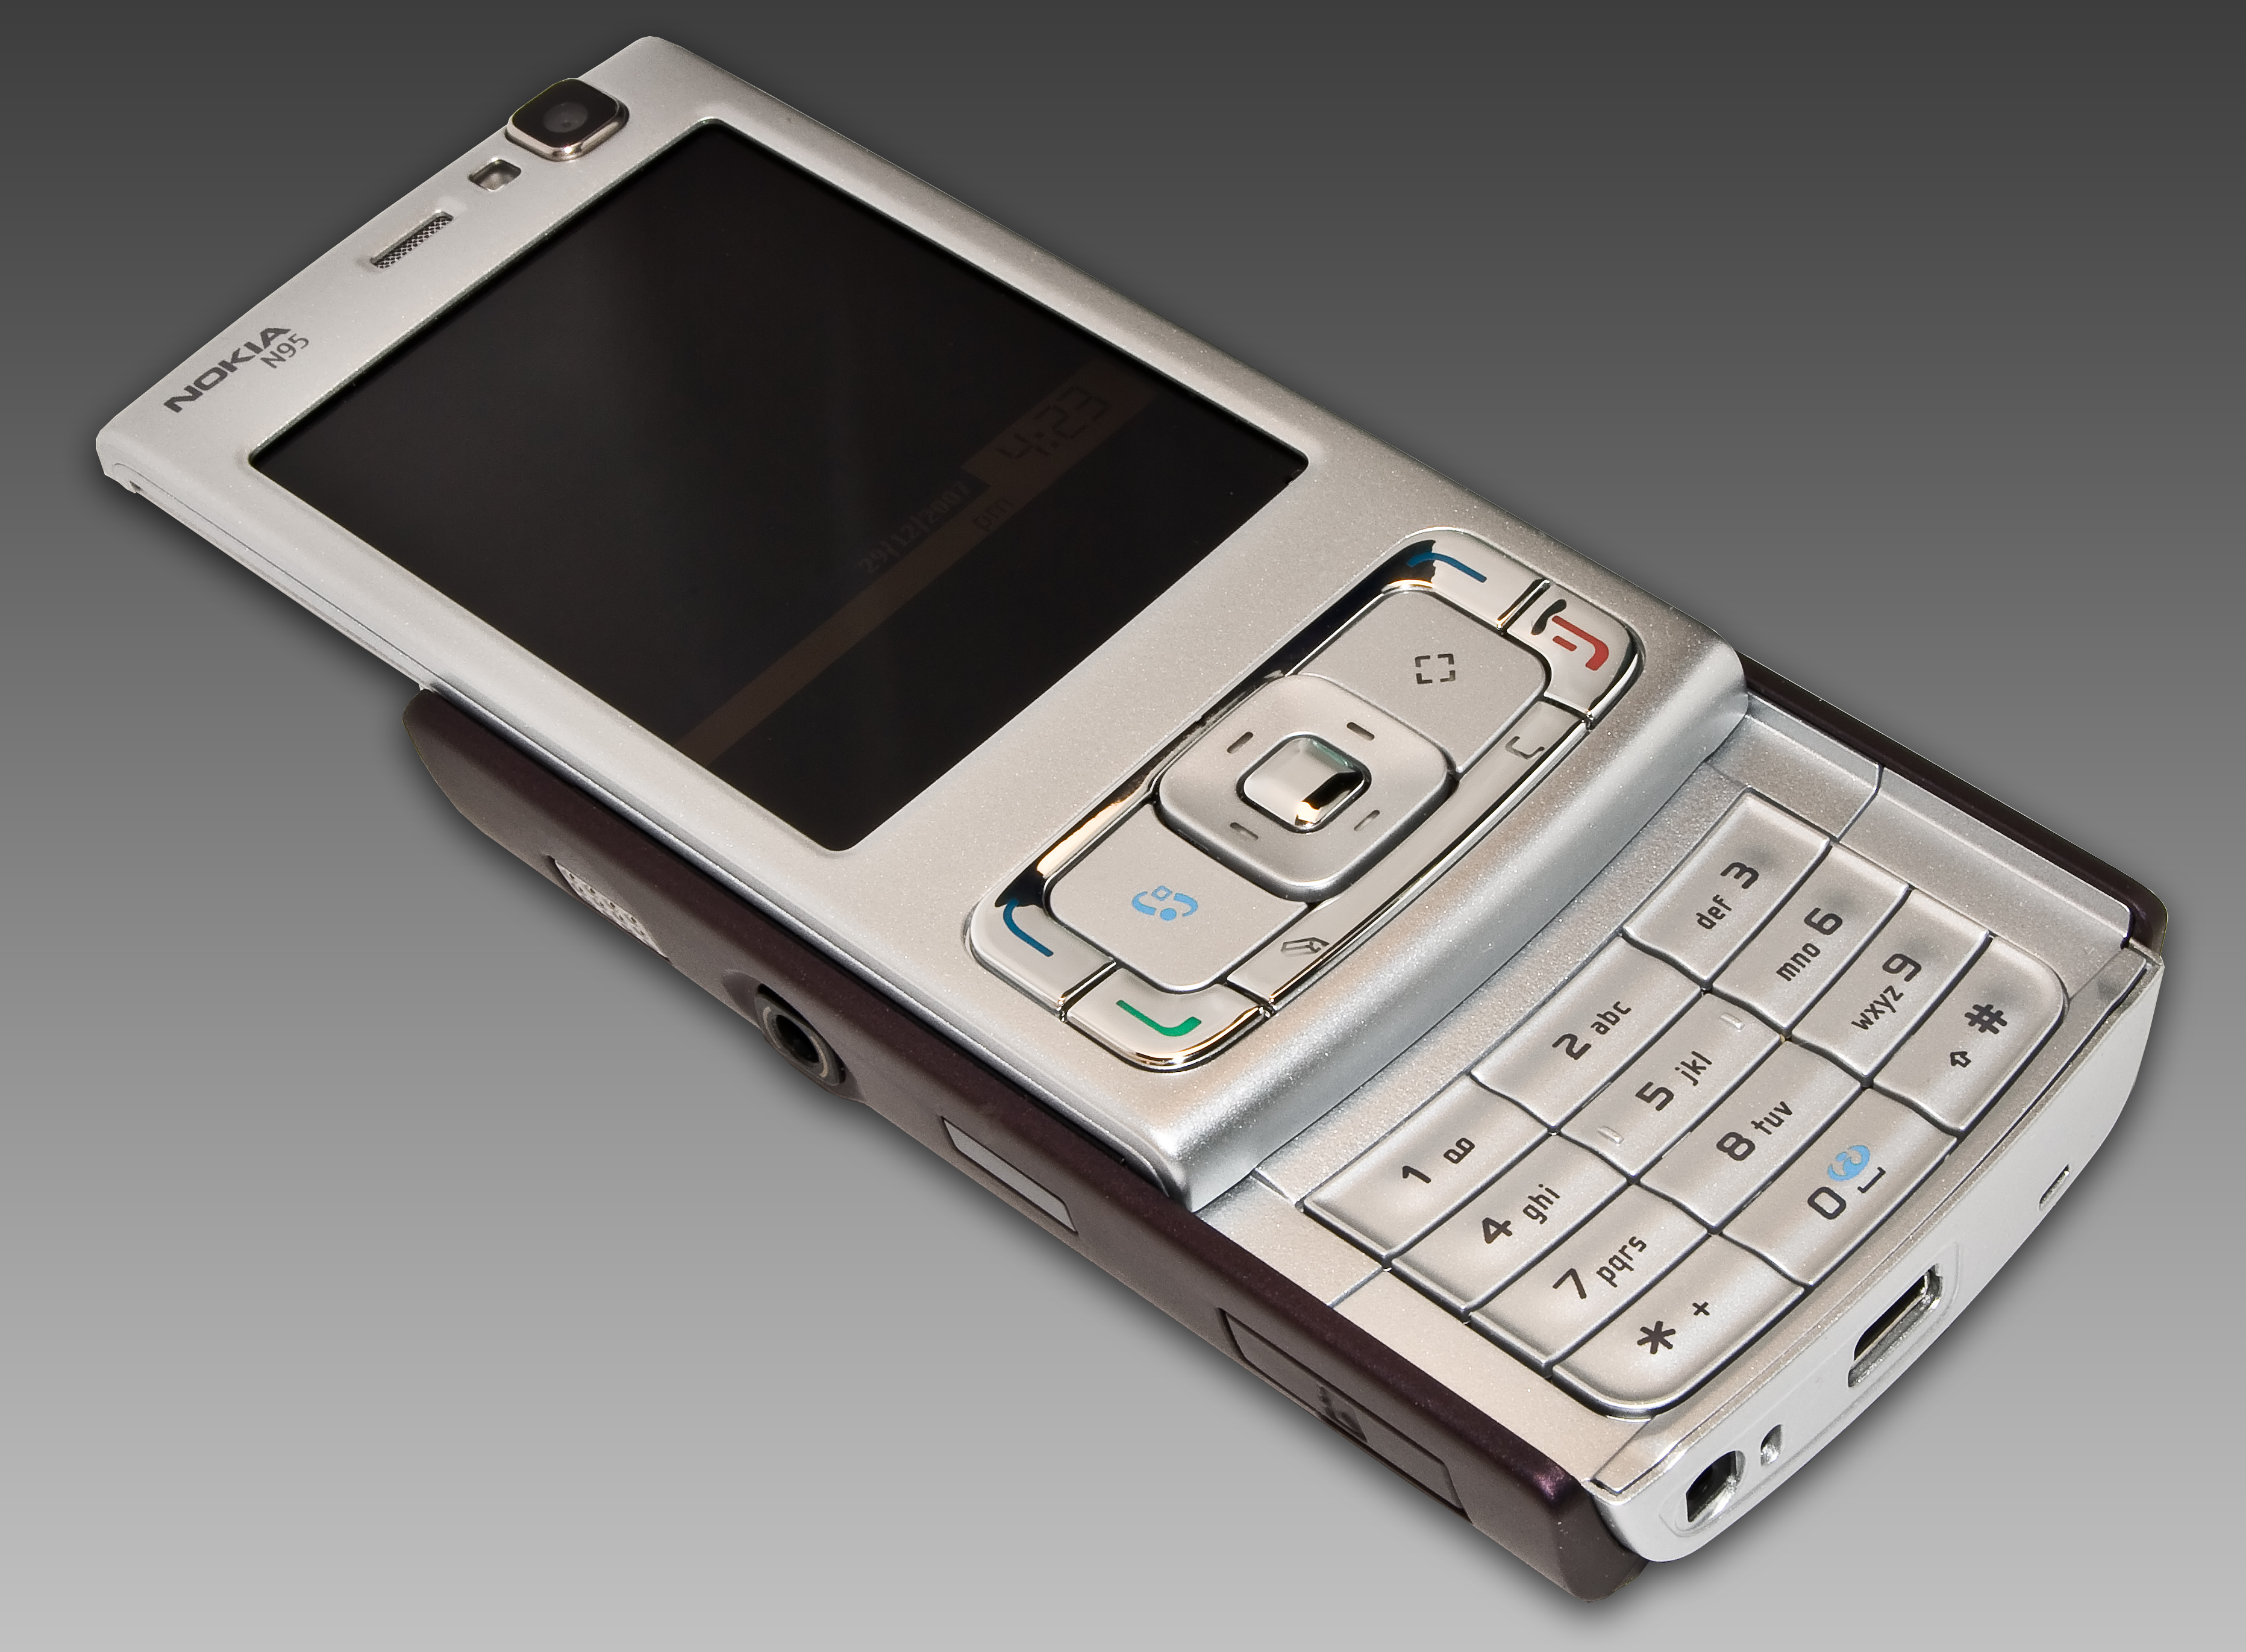
\includegraphics{images/N95_Front-slide-open}
    \caption{Nokia N95\cite{nokiaPhone}}
    \label{nokia}
\end{figure}

Notizen: \\

Work 1: "`StudentLife: Assessing Mental Health, Academic Performance and Behavioral Trends of College Students using Smartphones"'
48 Computer science students. 10 Wochen (ein Term)
Betrachtet Workload -> Stress, sleep, mood, \textbf{sociability}, activity, mental wellbeing und academic preformance.
Benutzt android.
Backup über wifi jedes mal wenn das handy geladen wird
"`During the collection phase, students were asked to respond to various EMA questions as they use their phones"'
Students werden per email benachrichtigt wenn die Daten ausbleiben.
The StudentLife app automatically infers activity (stationary, walking, running, driving, cycling), sleep duration, and sociability (i.e., the number of independent conservations and their durations). The app also collects accelerometer, proximity, audio, light sensor readings, location, colocation, and application usage.
Das handy schneidet ton mit und detectet conversationen.
A series of entry health and psycholog- ical baseline surveys are administered 
During the exit stage, we administered an exit survey, interview and the same set of be- havioral and health surveys
2014
\par

Work 2: "`Who’s Who with Big-Five: Analyzing and Classifying Personality Traits with Smartphones"'
83 french speaking switzerlanders over 8 months
Shown: aggregated features obtained from smartphone usage data can be indicators of the Big-Five personality traits
automatic method to infer the personality type of a user based on cellphone usage
75.9\% accuracy
Nokia n95 phone (bild!)
NEO FFI
gesammelte Features: calls (Call Logs), SMS (SMS Logs), bluetooth scans (BT Logs ), and application usage (App Logs ) (Nur Anzahl von öffnen, nicht zeit).
2011

\par
work 3: "`The Impact of Personality Traits on Smartphone Ownership and Use"'
312 participants
This study directly tests the effect of the "Big Five" personality traits on smartphone ownership and use.
We found that extraverted individuals were more likely to own a smartphone. Also, extraverts reported a greater importance on the texting function of smartphones
Age ranged from 18 to 77 years with a median age of 41 and a mean age of 40.
Respondents who owned a smartphone were then asked to rate on a five-point scale (1, not important at all, to 5, very important) the importance of six smartphone functions: phone calls, texting, internet, e-mail, music, and games. 
We measured personality with John’s (1991) Big Five Personality Inventory
2011

\par
Work 4: "`Personality and Self-Esteem as Predictors of Young People’s Technology Use"'
Participants were 200 university students (146 females, 54males)
Personality: The 60-item NEO FFI Personality Inventory + The 25-item Coopersmith Self-Esteem Inventory Adult Form
Self report: Time Spend on calls, sms and IM, and addictive tendencies towards those. 
2008

\par
work 5: "`Personality and self reported mobile phone use"'
112 participants in this study (78 females, 34 males). Age ranged from 18 to 59 years.
The Coopersmith self-esteem inventory
NEO-FF
selfreport- Mobile phone use survey



%%% Local Variables: 
%%% mode: latex
%%% TeX-master: "diplarb"
%%% End: 
